\documentclass[12pt]{zettel}

\renewcommand{\gregor}{\put(9.2,-3.5){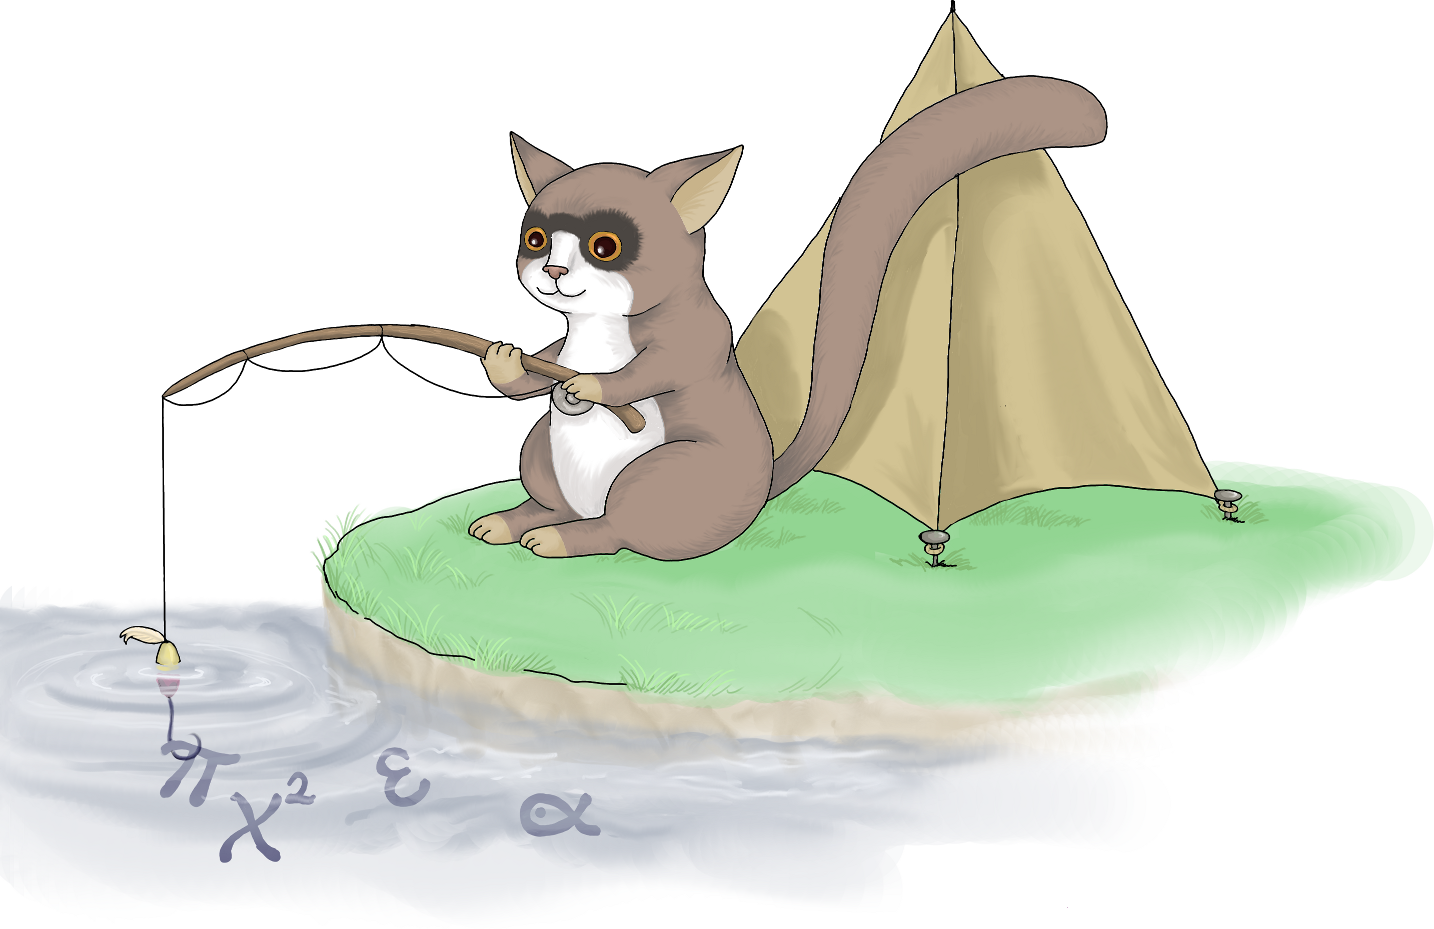
\includegraphics[scale=0.18]{campgregor}}}

\usepackage{framed}
\definecolor{shadecolor}{rgb}{.97,.97,.97}

\geometry{tmargin=1.5cm,bmargin=1.5cm,lmargin=2.0cm,rmargin=2.0cm}

\begin{document}

\renewcommand{\betreff}{Mathecamp -- schön war's!}

\makeletterhead{}
%\begin{picture}(0,0)
%  \put(7.0,-19.0){%
%    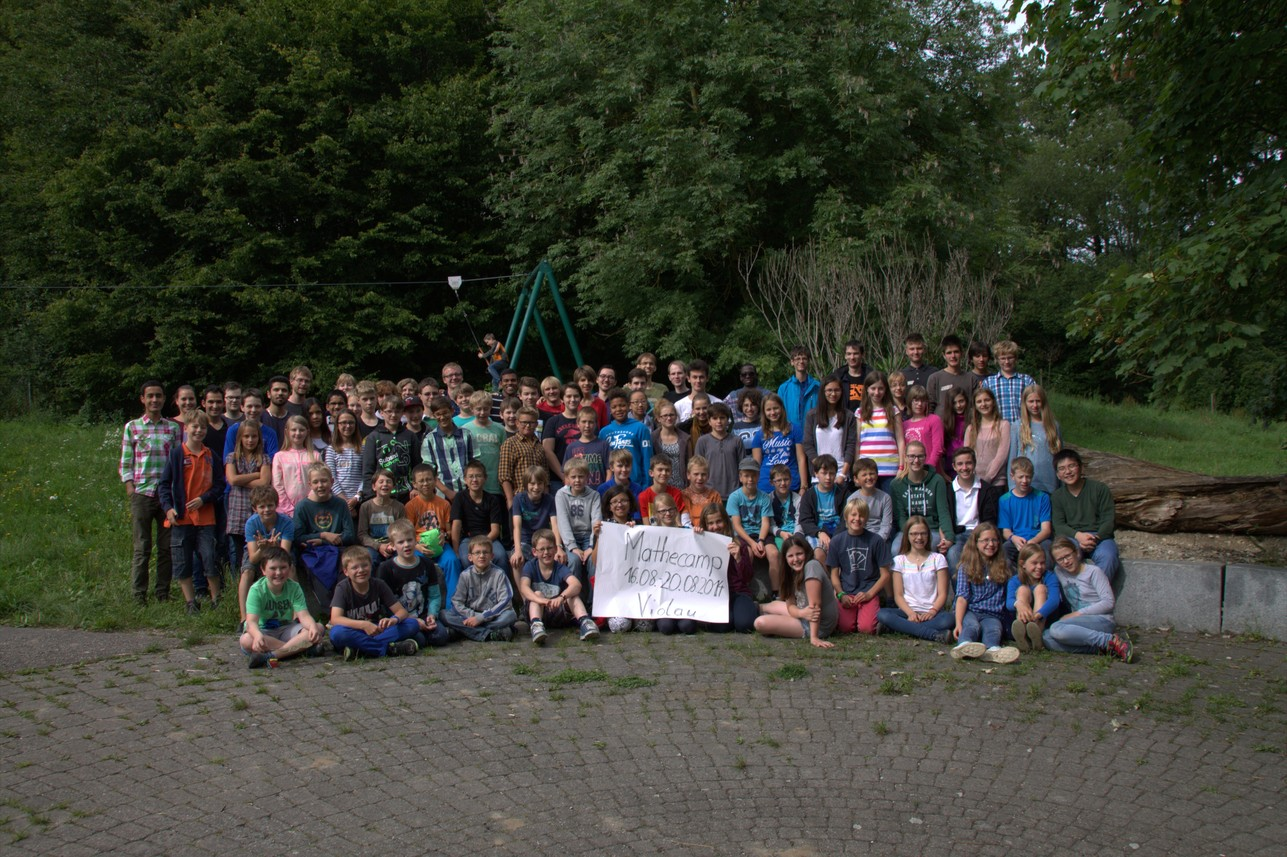
\includegraphics[scale=0.2]{gruppenfoto}
%  }
%\end{picture}
\vspace{-2em}

Liebe Schülerinnen und Schüler, liebe Eltern,

hoffentlich hattet ihr nach dem Mathecamp noch schöne Ferien und jetzt einen
guten Start in das neue Schuljahr! Wir hoffen, dass ihr nicht nur die
mathematischen Themen interessant fandet, sondern ihr auch rundherum viel
Spaß hattet. Uns hat das Camp mit euch sehr viel Freude bereitet.

Eine Fotogalerie findet ihr online unter \url{...} (Passwort \texttt{svenja}).

\begin{center}
  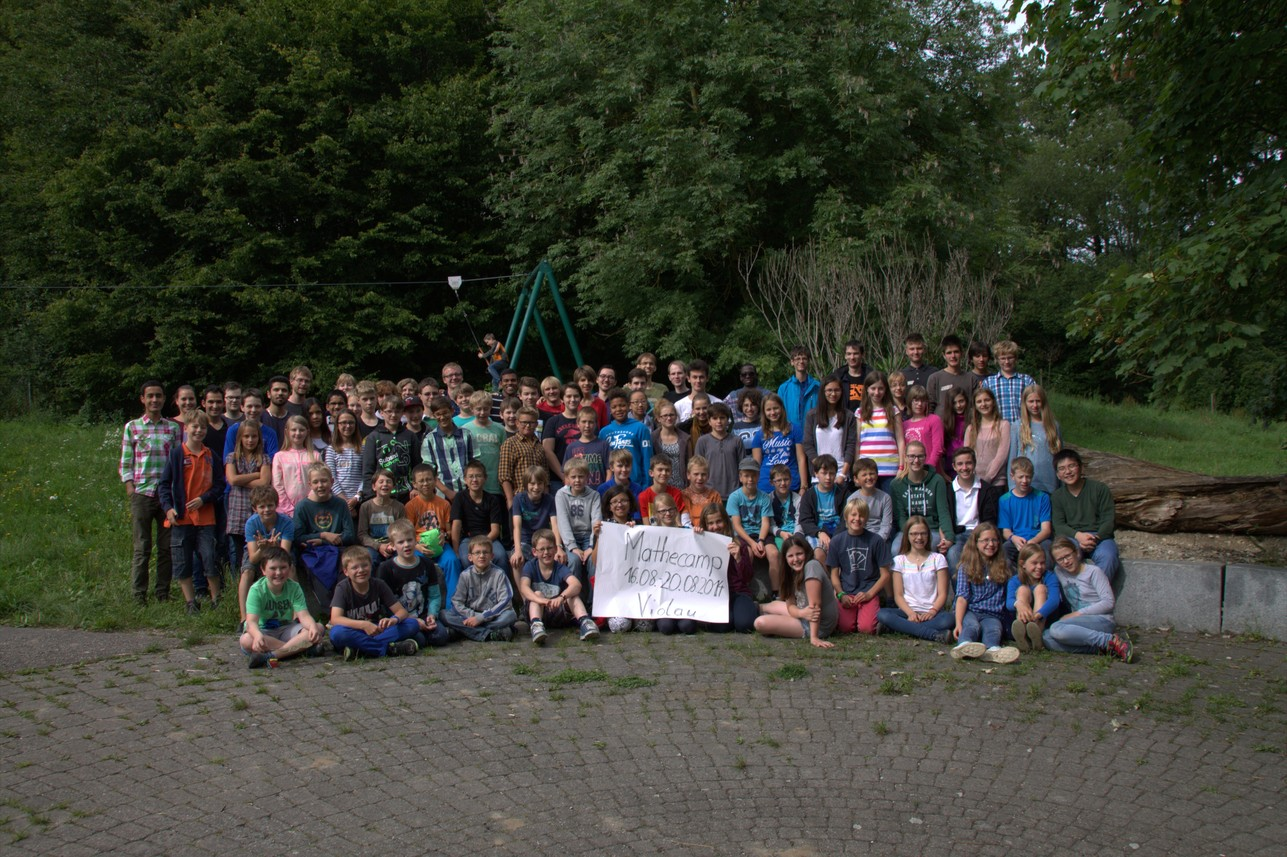
\includegraphics[scale=0.25]{gruppenfoto}
\end{center}

Nächstes Jahr werden wir das Camp wieder veranstalten -- euren Rückmeldungen
entsprechend dann voraussichtlich sieben statt nur fünf Tage. Diesbezüglich
werden wir euch rechtzeitig informieren. Natürlich hören wir auch gerne
konstruktive Kritik, damit wir das nächste Mathecamp noch besser
machen können, etwa die in diesem Jahr langwierige Zimmerverteilung.

Wir bedanken uns herzlich bei \emph{Bündnis für Augsburg}, dem
\emph{Mathematisch-Physikalischen Verein} und den Professorinnen und
Professoren der Lehrstühle für \emph{Algebra und Zahlentheorie},
\emph{Angewandte Analysis} und \emph{Nichtlineare Analysis} des Instituts für
Mathematik für ihre Unterstützung.
Besonderer Dank gebührt einem Professor des
Lehrstuhls für \emph{Analysis und Geometrie}, ohne dessen engagierten Einsatz
das Mathecamp nicht stattfinden hätte können.
Ferner bedanken wir uns bei Ihnen, liebe Eltern, für die zahlreichen
Spenden.

Wir wünschen euch viel Spaß und Erfolg im neuen Schuljahr und würden uns
sehr freuen, euch bei der Eröffnungsveranstaltung des Matheschülerzirkels am
18.~Oktober oder spätestens beim Mathecamp im nächsten Jahr wiederzusehen!
\emph{Euer Mathecamp-Team}

{\small Meru Alagalingam, Martin Baur, Ingo Blechschmidt, Tim Dafler, Philipp Düren,
Alexander Engel, Kathrin Helmsauer,
Christian Hübschmann, Jil Hümmer, Sven Prüfer,
Lisa Reischmann, Peter Uebele}

\end{document}
